\chapter{Theoretical framework}
Quantum computing is based on a general framework that does not depend on the physical platform. Here, important concept such as qubit, and quantum operations are described before showing how we can realize them, from a theoretical point of view, with trapped ions. The same goes with quantum networking, the concept and the realization can be treated separately and they will be described in this chapter. Furthermore, in this chapter we will take a look into Gaussian beams and their properties. Since that is the shape emitted by laser, it is important to understand their characteristic and how to manipulate them. Lastly Acousto-optical interactions are introduced and studied to give an idea of how AODs work and how they can be used to steer a laser beam.
\section{Quantum logic with trapped ions}
\subsection{Quantum computer and quantum gates}
The concepts of quantum computing are borrowed and extended from classical computational theory. In the classical case, information is represented in terms of binary digits, the so called bit, essentially mapping information to a base-2 number. Information processing is done with gates acting of those numbers. The idea of quantum computer is still to encode information in a binary form, but due to the nature of quantum mechanics, a quantum bit (in short qubit) gains new features that can be exploited to perform different kind of operations that in some cases are a speed up compared to the classical case.\\
A qubit is formally a normalized wave function that can be written as superposition of two orthogonal states indicated usually with $\ket{0}$ and $\ket{1}$:
\begin{equation}
\label{qubit}
\ket{\psi} = \alpha \ket{0} + \beta\ket{1},
\end{equation}
where $\alpha,\beta$ are probability amplitudes, two complex numbers that satisfy the relationship $|\alpha|^2+|\beta|^2 = 1$.
At first glance, the advantage of qubits seems obvious, while one classical bit can store only one bit of information, a qubit can be in any linear combination, i.e. $\alpha$ and $\beta$ can be chosen freely and any information can be represented. Although, the reality is different, due to rules of quantum mechanics, $\alpha$ and $\beta$ cannot be directly accessed, which means that we can get only a limited amount of information out of a qubit. The outcome of measuring a qubit will give the value 0 with a probability of $|\alpha|^2$ and 1 with a probability of $|\beta^2|$.  [..]

Qubits also have a geometrical representation that can be useful, equation \eqref{qubit} depends on 4 real numbers, however since $\psi$ is normalized, we can rewrite the expression as
\begin{equation}
\ket{\psi} = e^{i\gamma}\left(\cos\frac{\theta}{2}\ket{0} + e^{i\varphi}\sin\frac{\theta}{2}\ket{1}\right).
\end{equation}
the global phase factor $e^{i\gamma}$ can be left out, as it does not influence the measurement outcome. This leaves us with only two real number: $\theta$ and $\varphi$. A qubit is therefore representable with only these two numbers that we can chose to represent geometrically with normalized spherical coordinates. The so called Bloch sphere is depicted in figure \ref{blochsphere}, every point on its surface represents a different state of the qubit. Here qubit manipulation can be visualized as trajectories on the surface, which in some cases is very useful. The drawback of this representation is that it is limited to only one qubit, so it loses usefulness when dealing with multiple qubits.
\begin{figure}[H]
\centering
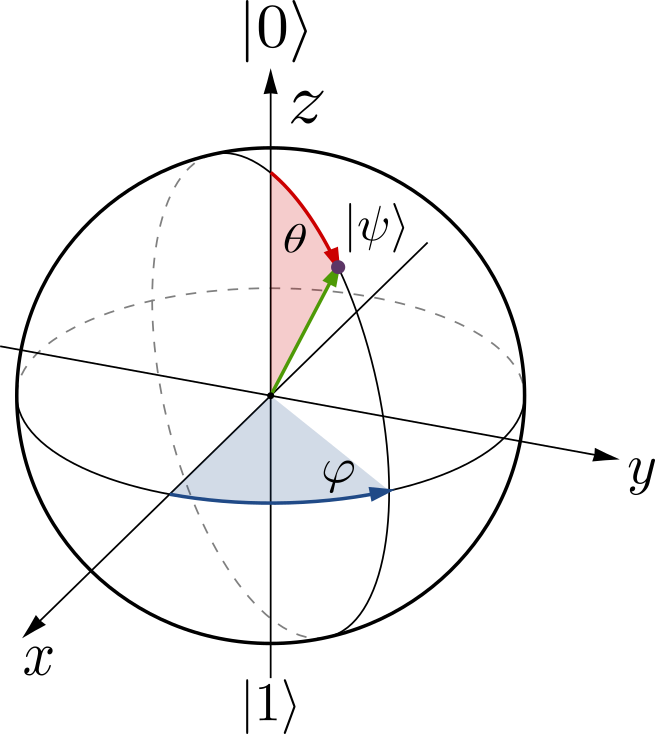
\includegraphics[width = .4\textwidth]{bloch_sphere}
\caption{The Bloch sphere. The states $\ket{0}$ and $\ket{1}$ are at the poles of the sphere, every other point of the surface represents a superpositions of these states. A quantum gate can be seen as trajectory on the surface mapping one state to another.}
\label{blochsphere}
\end{figure}

A more practical way of dealing with qubits is via matrices. We can assign to the states $\ket{0}$ and $\ket{1}$ the following:
\begin{equation}
\ket{0} = \begin{pmatrix}
 1 \\
 0
\end{pmatrix} \quad
\ket{1} = \begin{pmatrix}
 0 \\
 1
\end{pmatrix} \implies \ket{\psi} = \begin{pmatrix}
 \alpha \\
 \beta
\end{pmatrix}.
\end{equation}
In this representation, manipulations of qubits are easily calculated using $2\times2$ unitary matrices. These kind of operations are named \emph{quantum gates} and they are the building blocks of quantum computing. Every quantum algorithm can be written as a sequence of quantum gates and it is therefore important to understand them. For a single qubit any gate can be written as combination of two operations \cite{hempel}
\begin{equation}
U_z(\theta) =  \begin{pmatrix}
 e^{-i\frac{\theta}{2}} & 0 \\
 0 & e^{i\frac{\theta}{2}}
\end{pmatrix} \qquad U_\varphi(\theta) = \begin{pmatrix}
\cos\frac{\theta}{2} & -i e^{-i\varphi}\sin\frac{\theta}{2} \\
-ie^{i\theta}\sin\frac{\theta}{2} & \cos\frac{\theta}{2}
\end{pmatrix}.
\end{equation}
These two matrices can be seen as two different rotations in the Bloch sphere, $U_z$ is a rotation around the $z$ axis by the amount $\theta$, while $U_\varphi$ is a rotation on the $x-y$ plane around an axis tilted by $\varphi$. examples [H gate, phase gate]\\
\newline
As we have seen, a single qubit has already the advantage of superposition compared to classical case. When considering multiple qubits, we gain even more quantum mechanical features like entanglement. This phenomenon does not have a classical analogy and it is an extremely useful tools in quantum information.\\
In general a state with $N$ qubits is written as tensor product of the single qubit states $\psi_i$
\begin{equation}
\ket{\psi_N} = \ket{\psi_1}\otimes \ket{\psi_2}\otimes \cdots \ket{\psi_N} \equiv \ket{\psi_1\psi_2\dots \psi_N}.
\end{equation}
If we had to write out explicitly all the probability coefficients of $\psi_N$, we would need $2^N$ complex numbers. It is clear then why classical computer cannot keep up. $N$ bits can only give $N^2$ different combinations, while the Hilbert space of qubits is exponentially larger.\\
Now, let us consider only 2 qubits, a particular case would be
\begin{equation}
\ket{\psi} = \frac{1}{\sqrt{2}}\left(\ket{00} + \ket{11}\right).
\end{equation}
If a measurement is made on one of the two qubit and, for instance, the outcome is 0, the wave function collapses to the state $\ket{00}$, collapsing also the state of the other qubit, even if no operation has been directly performed on it. Next you measure the the second qubit and the outcome will be 0 with unitary probability. Viceversa, if the outcome if the first measurement was 1, the state collapses to $\ket{11}$ and the outcome of the second measurement is always 1. The two qubits are correlated, but this correlations is stronger than the classical one.\\
Gates that involve multiple qubits are written as $2^N\times 2^N$ unitary matrices, a famous example is the CNOT gate, [..]

It can be shown [] that the examples we saw here, H gate, phase gate, and CNOT gate form a universal set of quantum gates, i.e. a sequence of these gates approximate every other quantum gate.

\subsection{Ion qubits and laser-ion interactions}
Qubits can be encoded in any pair of orthogonal states. In the case of an ion it is possible to take two internal electronic states. The choices are multiple: an optical qubit is implemented in an optical transition, an hyperfine qubit is between two hyperfine states, and a Zeeman qubit can be realized with two magnetically separated levels. We will take the choice of an optical qubit, in this case lasers provide an easy way to manipulate the population of the two level and therefore to manipulate the state of the qubit, implementing quantum gates in an almost straightforward way. As long as the chosen levels are well separated, and the light is near resonant to the transition, it is possible to describe the system with the basic 2-level atom scheme interacting with classical light. \\
In this section, the theoretical model of a 2-level atom is presented together with a model of interactions between the laser and the ion. This represents a physical implementation of the concepts illustrated in the previous section.
\begin{figure}[H]
\centering
\includegraphics[width = .4\textwidth]{2levelatom}
\caption{2-level atom scheme, the ground and excited states are denoted as $\ket{g}$, and $\ket{e}$. $\omega_l$ is the laser frequency, which is detuned by $\Delta$ from the transition frequency $\omega_0$.}
\label{2levelatom}
\end{figure}

Consider the system in figure \ref{2levelatom}, the Hamiltonian of the atomic part can be written as:
\begin{equation}
H_a = \hbar\omega_0 \ket{e}\bra{e},
\end{equation}
where $\omega_0$ is the frequency difference between the ground and excited state, the energy of the ground state has also been set to 0. The Hamiltonian of the interaction between light and atom can be written as []
\begin{equation}
H_{int} = -d\cdot E
\end{equation}


- 2 level atom scheme\\
- Model of laser-ion interaction: rabi flops, AC stark shift
\section{Quantum networking with trapped ions}
\subsection{General introduction}
- Nodes, interface, link, protocols\\
- logic, memory, interface, Bell pairs, purification, multi-mode
- Distributed entanglement
\subsection{Cavity QED}
- Simple model atom in cavity: g,gamma, k
\section{Basics of ion trapping}
\subsection{Linear Paul trap}
- How a Paul trap works\\
- micromotion?
\subsection{Ion strings}
We have seen that the potential inside the trap can be described as an harmonic potential. It is then possible to calculate the ion separation between $N$ ion loaded in the trap. This will give us an idea of how narrowly the beam should be focused and will set an appropriate problem spatial scale.\\
We will consider only the $z$ direction where the ions are weakly confined and will form a string. The harmonic potential is then given by
\begin{equation}
V = \sum_{i=0}^N \frac{1}{2}M\omega^2z_i^2 + \sum_{i\neq j}^N\frac{Z^2e^2}{8\pi \epsilon_0}\frac{1}{|z_i-z_j|}
\end{equation}
The equilibrium position can be found at the minima of the potential, i.e. where the first derivative zeros
\begin{equation}
\frac{\partial V}{\partial z_i} = 0 \implies u_i - \sum_{j=1}^{i-1} \frac{1}{(u_i-u_j)^2} + \sum_{j= i+1}^{N} \frac{1}{(u_i-u_j)^2}= 0,
\end{equation}
where we defined the dimensionless quantity $u_i = z_i/l$ and $l^3 = \displaystyle\frac{Z^2 e^2 }{4\pi \epsilon_0 M\omega^2}$.
The last equations can be solved analytically only for 2 or 3 ions. In fact, for the case $N=2$ we simply get the system
\begin{equation}
\begin{cases}
  u_1 + \frac{1}{(u_1-u_2)^2} = 0\\
  u_2 - \frac{1}{(u_1-u_2)^2} = 0
  \end{cases} \quad \implies \quad u_1 = -u_2,\quad  u_1 = \left(\frac{1}{2}\right)^{2/3} \simeq 0.629
\end{equation}
For calcium-40 ions in a Paul trap with axial confinement of 1MHz, we have $l \simeq 4.45\times 10^{-6}\, \mu$m, which means that 2 ions are separated by $\simeq 5.6\, \mu$m. In the case of more ions the separation is lesser with the same confinement, but it is also possible to lower the axial frequency and increase the separation between the ions such that also in the case of several ions, the distance between them is still in the order of several $\mu$m. This size is accessible with current focusing optics and it is above the diffraction limit.\\
For more ions, a numerical approach has to be used, \cite{ion_spacing} reports values of $u_i$ up to $N=10$, and gives an empirical formula of the minimum separation
\begin{equation}
u_{min}(N) \simeq \frac{2.018}{N^{0.559}}
\end{equation}
\subsection{Doppler cooling and detection}
\section{Laser beam}
\subsection{Gaussian beams}
Lasers emit light in the shape of Gaussian beams, so it is import to understand what Gaussian beams are and their characteristics. In this chapter we will take a closer look into such beams and introduce important quantities to characterize a Gaussian beam. \\
From a theoretical point of view, Gaussiam beams are solution of the Helmholzt equation
\cite{saleh}
- Introduction to import quantities, like FWHM, focus, waist!
\subsection{Diffraction limit}
- To search whats limiting the diffraction, (lambda/2)
\subsection{Beam stearing via AOD's}
- How AODs work, simple Model\\
- Introduce diffraction efficiency, bandwidth
